\documentclass[a4paper]{article}

\usepackage[english]{babel}
\usepackage[utf8]{inputenc}
\usepackage{amsmath}
\usepackage{graphicx}
\usepackage[margin=2.5cm]{geometry}
\usepackage{url}
\usepackage{hyperref}
\usepackage{lmodern}
\usepackage[T1]{fontenc}
\usepackage{array}
\usepackage{booktabs}
\usepackage{subcaption}
\title{Integrating touchless gesture based navigation into the modern desktop experience}

\author{
    David Liskevich 
  }

\date{}


% END PREAMBLE %%%%%%%%%%%%%%%%%%%%%%%%%%%%%%%%%%%%%%%%%%%%%%%%%%%%%%%%%%


\begin{document}
\maketitle

\begin{description}
\item [\centering Interim Report]
\end{description}

\newpage

\tableofcontents
\newpage

\section{Introduction}
There is a constant challenge in modern computing to provide an intuitive user interface , with modern developments coming as much from new software, as using new hardware. Touch-screens and touch technology are currently the standards for new intuitive devices. It reduces the need for moving between both a mouse and a  keyboard, allowing users to navigate in a natural manner using their hands. The next logical step, is to dispense the need to touch anything but to intuitively use your hands to navigate and use applications. It's far easier for a user to just point at what they want to do, or gesture in a way that  makes sense to that user to achieve particular results. There's many existing sectors where this would be advantageous such as a hospital, where hygiene is of the utmost concern or any public computer for that matter. \\ \\While there are many devices that implement some form of human tracking for novel purposes (e.g. the xbox Kinect),The Leap, by LeapMotion, is a device specifically  designed to monitor motion and track hands in a roughly  hemispherical shape above it to around 1m in area while it is on a desk. The Leap can detect finger positions up the closest 0.01mm\cite{accuracy} and has the capability to track the positions of individual bones in the hand using 3000 frames per second.\\ \\ The official software provides not only the service to capture information from the Leap, but also APIs in many popular languages. The software has many in-built functions for obtaining hand tracking information , but it only has 4 predefined gestures. There have been attempts to implement desktop navigation with it, predominately on Microsoft Windows, but they have been applied to existing operating systems and user interfaces, user interfaces which were designed to be used with traditional computer control, a keyboard and mouse. The reason touch-screen technology has been successful is that the operating systems and user interfaces were designed with touch technology in mind, if one attempted to operate Microsoft windows XP with touch-screen technology, the result would most likely be a clumsy and difficult experience. For a truly intuitive experience the user interface/GUI of the operating system would need to be designed with the Leap in mind. \\ \\The existing implementations,both open-source and private, using the Leap have also been hindered by the limited number of gestures readily recognized by software. To have a truly intuitive system, users or developers need to be able to define whatever gesture they feel most intuitive for an action. The entire experience suffers further when one considers that any application didn't have the Leap in mind; One can only navigate as if one is using mouse,where it may be more intuitive to have a gesture perform an action. \\ \\How about: The potential for an eco-system of applications and usages for the Leap in traditional desktop settings is being squandered. This is not only due to the limited inbuilt capacity of the device, but also due to a lack of knowledge regarding it's APIs from developers intending to integrate Leap into their applications Open-source development could accelerate the growth of the modern desktop experience by. \\The idea of this project is to try and solve these issues by extending the gesture support of the Leap, creating a desktop environment designed specifically for it to allow other developers(or users) to very easily integrate Leap gestures into their applications.
\newpage
\subsection{Objectives}\label{Objectives}
The main objectives I set out to achieve, in order of priority are: 
\begin{enumerate}
\item Implement a new gesture recognition scheme/library for the Leap that can handle custom gestures
\item Implement a method of assigning gestures for existing applications so that applications that weren't designed to be used with the Leap can still be used intuitively 
\item Integrate the gesture recognition and training into an existing desktop environment to allow navigation of it using the Leap
\item Tailor the arrangement and aesthetics of the desktop environment so that is intuitive and accurate to navigate it using the Leap
\item Remove the need for a keyboard by creating an on-screen implementation for use with the Leap
\item Create custom necessary applications for the desktop environment that are designed specifically for desktop navigation using the Leap, examples include a file browser, and Internet search
\item Implement some method of altering the appearance of the user-interface of existing applications so that they are arranged with touch-less navigation in mind
\end{enumerate}
\newpage
\section{Background}
\subsection{The Leap}
The Leap Motion controller is a small USB peripheral, 13mm X 13mm X 76mm device which is designed to be placed on a physical desktop, facing upward. Using two monochromatic IR cameras and three infrared LEDs, the device observes a roughly hemispherical area, to a distance of approximately 1 meter (3.28084 feet). The LEDs generate a 3D pattern of dots of IR light and the cameras generate almost 300 frames per second of reflected data. This is then sent through a USB cable to the host computer, where it is analyzed by the Leap Motion controller software.\cite{Leap Teardown}\cite{Leap Specs}

The optical sensors are directed upward and have a field of view of about 150 degrees with the effective range extending between 1" and 2 ft. \cite{Leap Overview} \\
\newline
\begin{figure}[htb]
\centering
\begin{subfigure}{.5\textwidth}
  \centering
  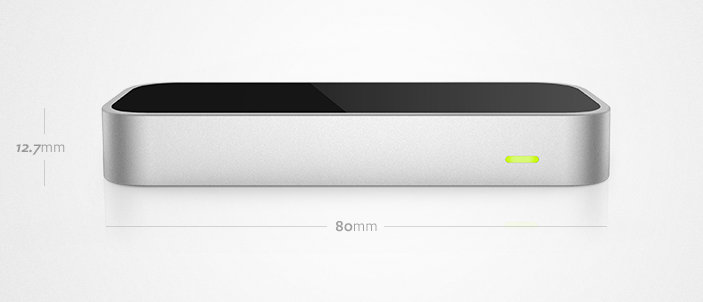
\includegraphics[width=.65\linewidth]{leap_01.jpg}
  \caption{Official photo of the Leap with dimensions \cite{Leap Site}} 
 
\end{subfigure}%
\begin{subfigure}{.5\textwidth}
  \centering
  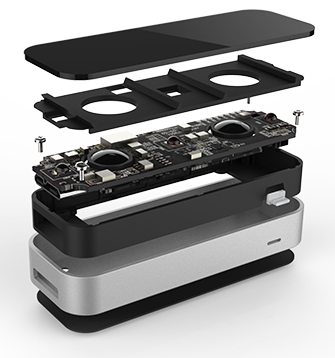
\includegraphics[width=.65\linewidth]{Leap_03.png}
  \caption{Disassembled view of the Leap \cite{LeapLab}}
 
\end{subfigure}
\end{figure}

	
\subsection{Leap Software}
\subsubsection{Skeletal Model and API}
The software use a proprietary algorithm which synthesizes 3D position data by comparing the 2D frames generated by the two cameras.\cite{Leap Specs}
\\ Integral to the software is the inbuilt hand tracking. As of version 2, the software operates on a detailed skeletal tracking model. See  figure \ref{skeletalModel}. \\

\begin{figure}[!h]
\centerline{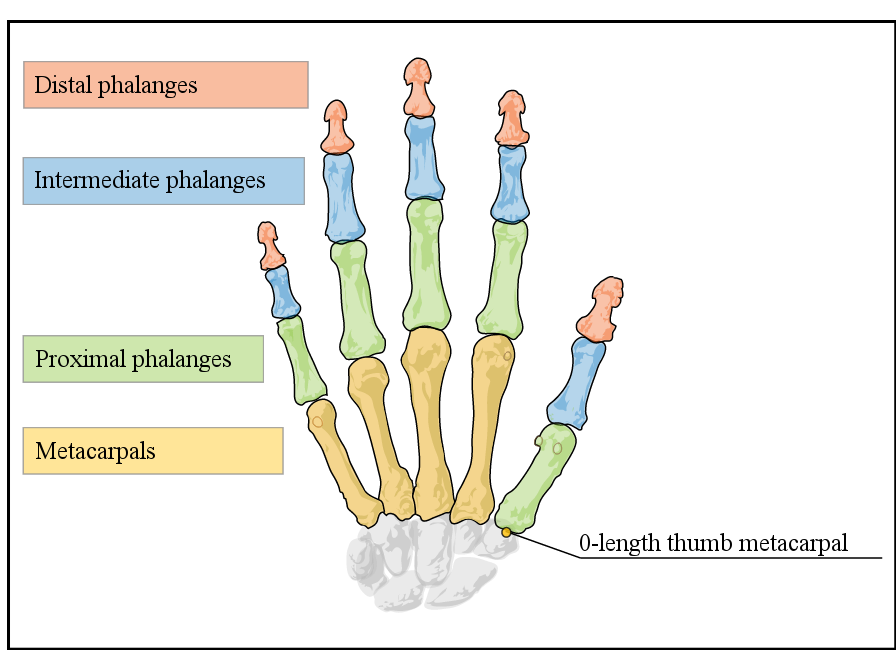
\includegraphics[width=0.3\textwidth]{skeletal.png}}
\caption{Skeletal hand model used by the Leap motion software and API
\label{skeletalModel}\cite{skeletalGuide}}
\end{figure} 
Using the new model,  better prediction of the position of fingers and hands which may not be perfectly in view have been achieved, improving persistence of hands in applications using the Leap. It allows for far more detail about the hand to be obtained, and I believe maximising the amount of data used in the gesture model will be integral to improving the gesture support.\\\\\\
As well as this, the software allows :\\
\begin{itemize}
\item Reporting a confident rating on the observed data
\item Identification of whether it is the left or right hand
\item Identification of individual digits
\item Reporting of position and orientation of each finger bone and identification of whether the finger is extended or not
\item Reporting of grip factors indicating if the user is pinching or grasping
\end{itemize}\cite{skeletalGuide}

The API provides access to a finger class, which will contain 4 bone objects, each of which has details about it's position and direction available for use. It also provides a pointable class, which contains both fingers (which at that moment are near straight) and thin long objects like pencils, which are modelled as tools. \\ \\
The software uses a right-handed Cartesian coordinate system, with the origin centered on top of the center of The Leap Motion Controller. As can be seen on figure \ref{coordinateSystem} 

\begin{figure}[!h]
\centerline{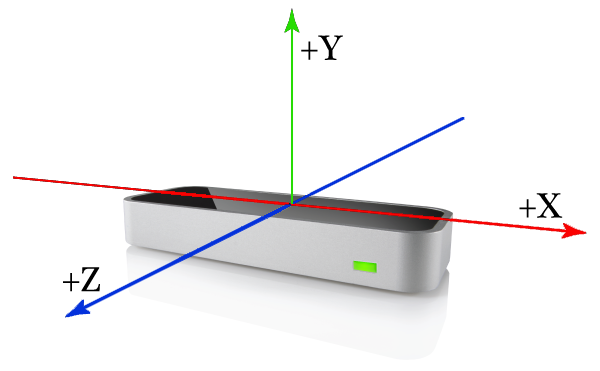
\includegraphics[width=0.4\textwidth]{Leap_Axes.png}}
\caption{Coordinate system used by the Leap motion software
\label{coordinateSystem}\cite{skeletalGuide}}
\end{figure}

Inherently, the API measures distance in millimeters, Time in microseconds, speed in millimeters/second and angle in radians. \\ \\

The motion tracking data is presented in the form of Frame objects, which in turn contain information about the hands in view, with data about each finger of those hand objects. The normal vector from the palm of each hand, and the direction the hand is facing are also recorded.\\ \\ Access to raw sensor images is also available, and contains the measured IR brightness values and calibration data. It could be interesting to try and calibrate the system using this data. 

\subsubsection{Operating system support}
The Operating systems officially supported by the Leap are Windows 7 or 8, Mac OS X 10.7 Lion and Ubuntu 12.04 LTS or later. Having investigated this claim on various forums, there is a disparity in the amount of support actually received. While Windows gets regular updates and robust support for the SDK, with Mac OS X getting similar if slightly slower support, the support for Linux is very poor. The leap store is not accessible on Linux and the leap daemon requires administrator privileges from a terminal to launch it, hardly enticing for potential users and developers. Due to this project involving the need to tailor a front end for use by the Leap, and both Windows and Mac OS X being fairly closed of in customisation, I will choose and focus on Linux as my platform. The inherent open-source nature and structure of the Linux operating system make it ideal for this kind of project, and for one I can help address the lack of a Leap-Linux Ecosystem
\subsection{OpenLeap software}
OpenLeap is an intitiative to encourage open-source development for the Leap Motion controller. \cite{OpenLeapProject}\cite{OpenLeapSite}

The have a number of projects contributed, some of which involve desktop navigation or mouse navigation using the Leap, we'll be looking at these in section \ref{NavigationExamples}. Their first project is the most ambitous however as it aimed to create an open-source driver, due to the poor linux support for the official driver \cite{OpenLeapDriver} \\
Through capturing the initlisation of the Leap and creating a script to replicate this, they have managed capture raw data from the Leap, and display the frames captured. However this includes no tracking of any kind, as such, this driver is very "raw" and use of it would require writing the rest of the driver myself and would require experience with low-level programming. This driver is not suitable for use other than grabbing the raw images. This means the official driver and daemon must be used for the project.
\subsection{Gestures}
\subsection{Definition of a Gesture}
It is important to first understand what we mean by a gesture.A gesture is most often defined as a predefined movement pattern, which has a definitive start point and end point i.e. they are finite. This is opposed to a continous gesture which is a predefined movement pattern that doesn't have a finite end point \\ The last type of "gesture" would be a pose, a predefined arrangement of the hand without movement in physical space that lasts above some minimum amount of time. \\ \\
As well as having multiple methods of defining the definition and model of a gesture, there are multiple ways of recognizing the start of a gesture. Given that for the purpose of this project, the leap will constantly reading in tracking data, there must be an accurate and efficient way of differentiating from any other free movement. The most common method is to define a minimum speed for the fastest moving part of the hand beyond which gesture recognition is triggered. \\
\subsection{Existing support}
The official Leap Motion software supports gestures, 4 specifically. These are (as can be seen in \ref{4Gestures})\\
\begin{figure}[!h]
\centerline{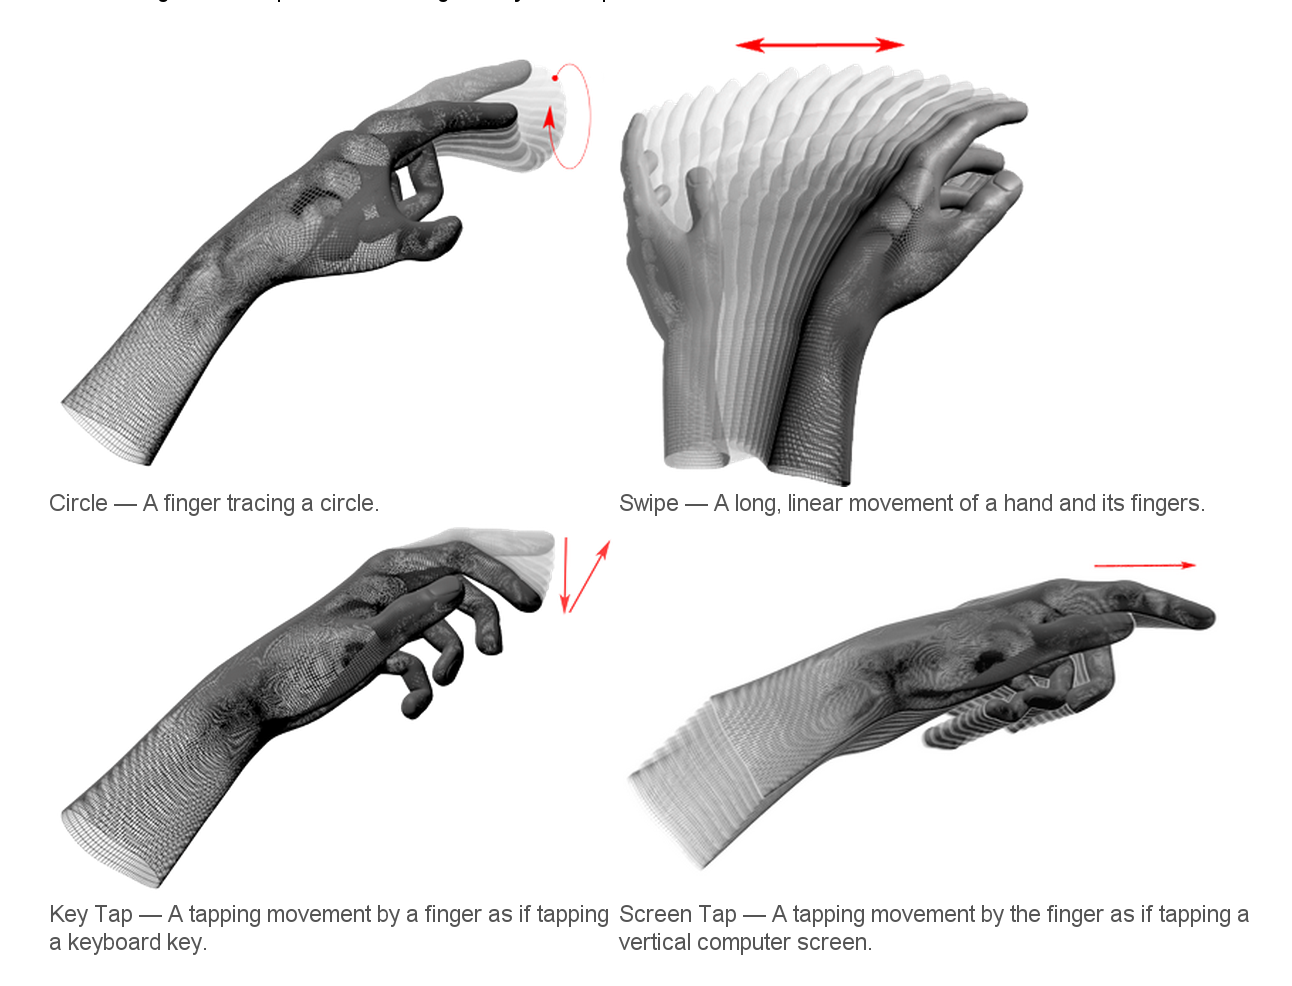
\includegraphics[width=0.6\textwidth]{4Gestures.png}}
\caption{Gestures officially supported by The Leap Motion Controller}
\label{4Gestures}\cite{Leap Overview}
\end{figure}
There is no support for defining custom gestures, so one has to have knowledge of the API to develop the ability to do this.
\newpage
\subsection{Algorithms and methods}
There are many algorithms that have been used successfully for recognizing gestures, some specifically for the LEAP:
\begin{description}
\item[Geometric template matching]{\label{GMT}\hfill \\
Geometric template matching uses recordings of the known gestures with large feature sets by first resampling them and making them the same length. The crux of the algorithm is that it takes time away as a factor. Gestures are modelled based on clouds of points which represent position in 3-d Space. The algorithm recnoizes gestures starts based on speed of movement i.e. once the hand moves fast enough, a gesture is considered to have begun. The clouds of points make the algorithm more robust to different users with different speeds or perhaps even users doing gestures in reverse order, the uncertainty is built into the model so as to account for "sloppy gestures". It is implemented in \ref{LeapTrainer} and is based on \cite{P}.

For actual recognition, a case-based approach is taken. The recognizer calculates a euclidean distance function for an entire gesture, comapres it to existing gestures and returns the one with the smallest distance. It uses a heuristic to resample points in a gesture and account for the gesture being performed in any order to allow different users to perform the same gesture slightly differently.
}
\item[Artificial neural-networks(ANNs)]{\hfill \\
ANNs are a supervised learning model used to mimic the brain of a living creature. Based on a large number of inputs through training data with examples, parameters are optimised until the large number of inputs can be classified into a result. There is a whole family of different algorithms/models that fall under this category or are used inside it in variations of it. The key of the system to to go through a large learning period to make it robust and reliable.\\
Hidden Markov Models(HMMs) are a variation which appear to be the most popular in use of gesture recognition. They are a statistical model containing hidden states that affect the stochastic pipeline but only a statistical estimate of their result is known
}
\item[Cross-Correlation]{\hfill \\
A simple algorithm which performs simple calculations based on the gemoetrical data of saved gestures and the currently performed one. It compares the performed gesture against all gestures and calculates and average correllation serious to find the closes match (if any)}
\item[Support Vector Machine]{\hfill \\
This is another supervised learning algorithm which seeks to model classes to be as distinct as possible while keeping the error that arises from unseen patterns lower. It is known to be difficult to establish the correct parameters, and said parameters may only work for a specific problem.
}
\end{description}
\newpage
\subsection{Open-source Gesture library implementations}
There have been a few different open-source implementations of gesture libraries, using various different recognition algorithms and on various different platforms. I will focus on those that were not built specifically for either Mac OS X or Microsoft Windows. 
\subsubsection{LeapTrainer.js \label{LeapTrainer}}
LeapTrainer.js is a gesture training and recognition framework using the Leap Motion JS API.
It employs various different gesture-recognition and recording algorithms to choose from:
\begin{itemize}
\item Geometric template matching
\item Cross-correlation
\item Neural-networks
\end{itemize}

It comes with a web-based user interface to train new gestures and tweak parameters in the classifier. By default it implements Geometric template matching of the form described in the \$P recognizer \cite{P} . The algorithm has been extended to account for gestures in 3-dimensions and tweaked for performance with the Leap. \\ \\
Alternatively it comes with a fully featured neural networks framework for training and recognition.

\begin{figure}[!h]
\centerline{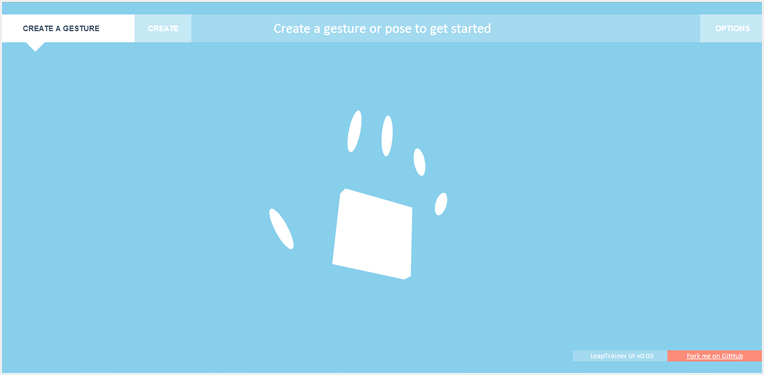
\includegraphics[width=0.5\textwidth]{leaptrainer-ui.png}}
\caption{LeapTrainer training ui}\cite{LeapTrainer}
\end{figure}

\begin{figure}[!h]
\centerline{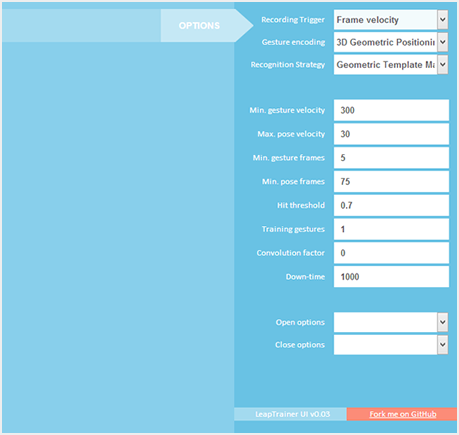
\includegraphics[width=0.4\textwidth]{training-ui-config.png}}
\caption{LeapTrainer training ui config}\cite{LeapTrainer}
\end{figure}
 This software was produced in 2013 and as such, uses the first version of the Leap software. This means it doesn't capitalise on the new detail found in the skeletal hand model. However even without this model, it's able to achieve quite robust and accurate performance. Both static poses and dynamic gestures are supported.\newpage
\subsubsection{Gesture Recognition Toolkit \label{GRT}}
The GRT is a multipurpose gesture recognition library employing many different algorithms :
\begin {itemize}
\item Adaptive Naive Bayes Classifier
\item AdaBoost
\item K-Nearest Neighbor Classifier
\item Decision Tree
\item Dynamic Time Warping
\item MinDist
\item Support Vector Machine
\item Artificial Neural Network (Multi Layer Perceptron)
\item Linear Regression
\item Logistic Regression
\item Multidimensional Regression
\end{itemize}
It provides both an extensive C++ api and a standalone graphical application. It supports both static poses and dynamic gestures and is compatible with any data input. It also performs regression, in real time it maps an input signal to an output signal, allowing finer details such as the angle in hands to manipulate objects on screen.
It comes with a vast number of filtering algorithms and statistical functions to take advantage of as well. \\ \\
\begin{figure}[!h]
\centerline{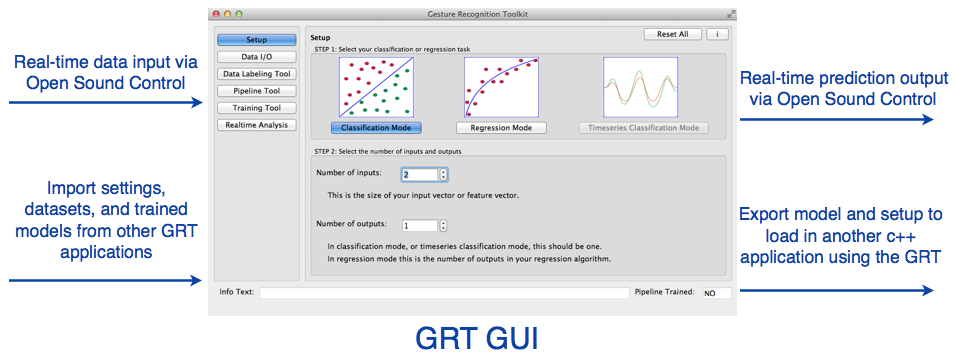
\includegraphics[width=1\textwidth]{grt.png}}
\caption{GRT}\cite{GRT}
\end{figure}
\newpage


\subsection{Desktop Environment}
\subsubsection{What is a Deskop environment}
A desktop environment is the implementation of the metaphor of using your computer like a real desk. It consists of a set of utilities and programs with a shared graphical user interface (GUI) . They provide icons, windows,folders, taskbars and generally all common GUI elements. Most importantly, they contain the window manager, a piece of software which controls the placement and appearance of windows in the system and the application launcher which provides a shortcut to all the users applications. \\ \\
\subsubsection{GNOME}
The GNOME desktop environment is one of the olderst open-source projects, operating under the Gnome project\cite{Gnome}.  
\begin{description}
\item[Design Principles]{\hfill \\
It's design principles are perfectly in tune with goal of this project and aims to be simple and intuitive to use. It aims to be minimilist, with only a thin tasbar showing when in an application is running, enabling a user to make use of the entire display space.

\begin{figure}[!h]
\centerline{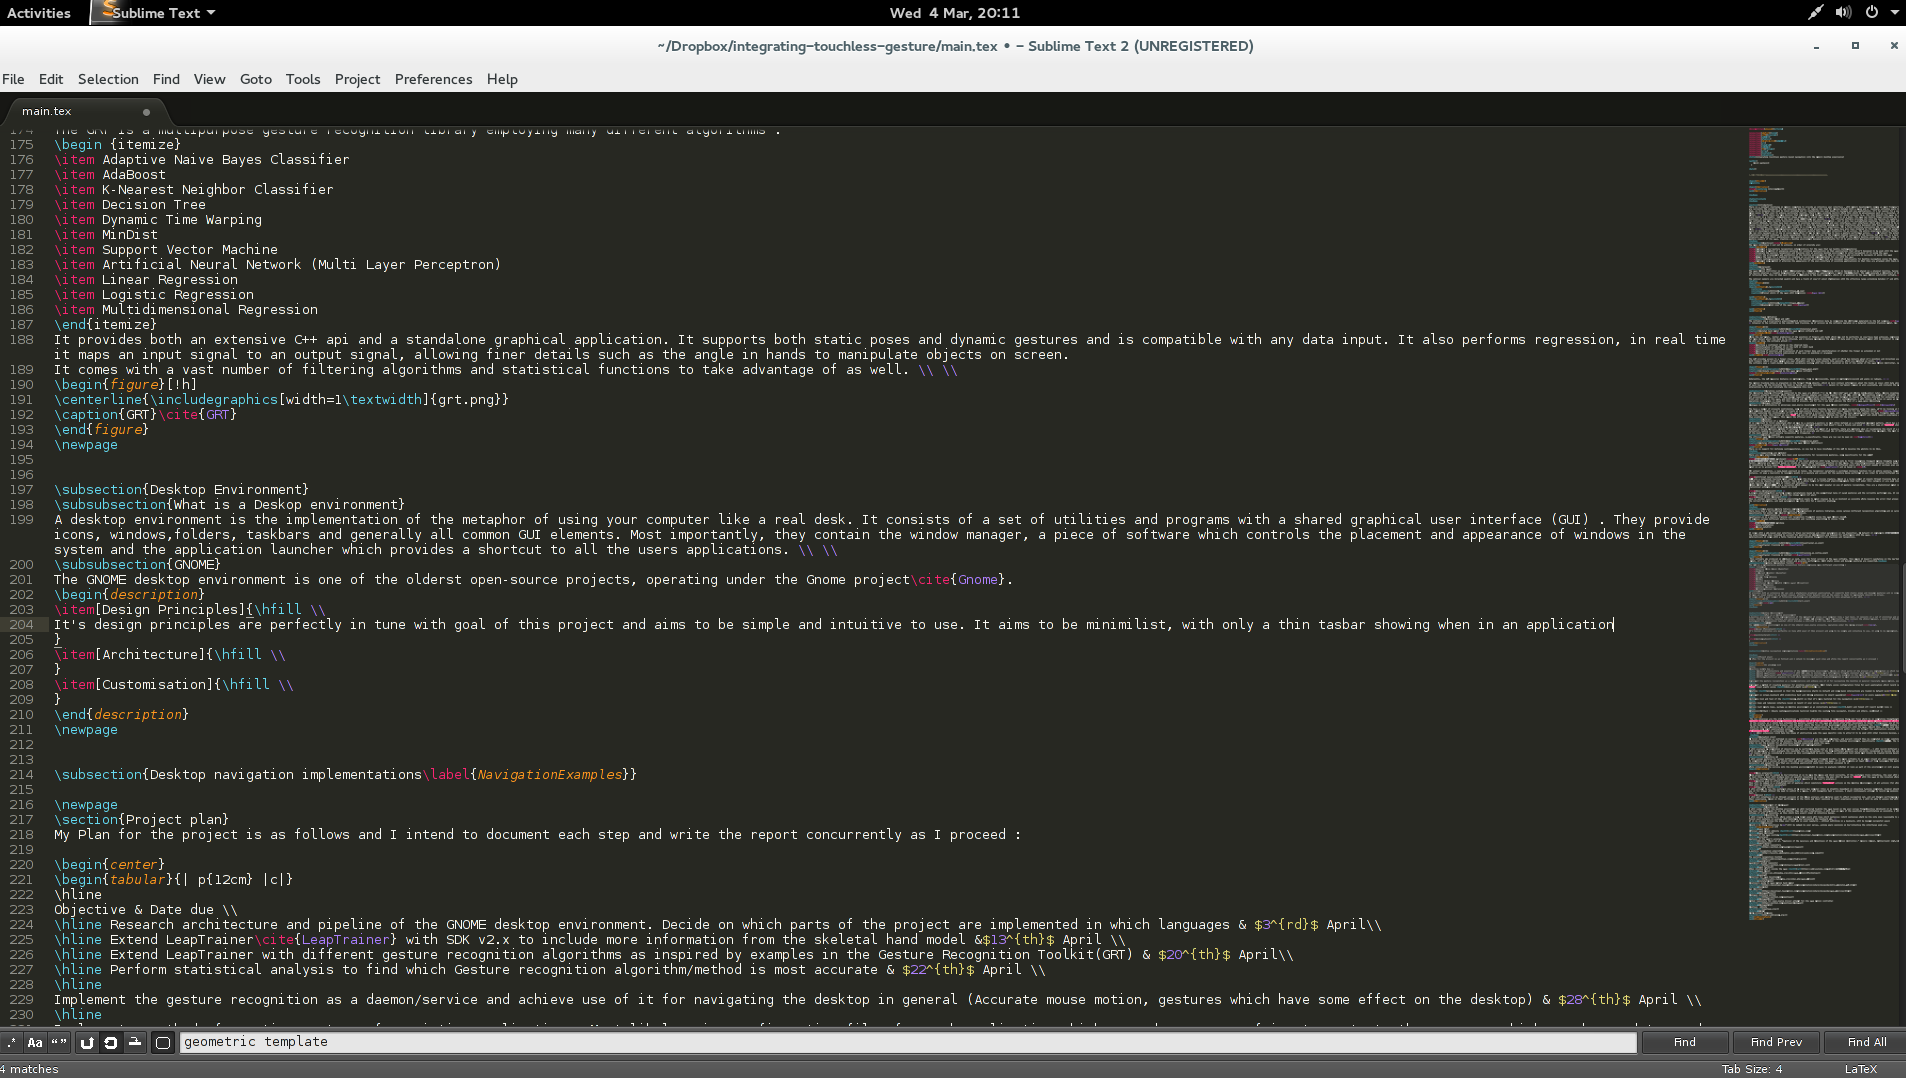
\includegraphics[width=0.65\textwidth]{Gnome.png}}
\caption{Gnome running an application}
\end{figure}

It provides a clean overview of running applications and favorite applications.
\begin{figure}[!h]
\centerline{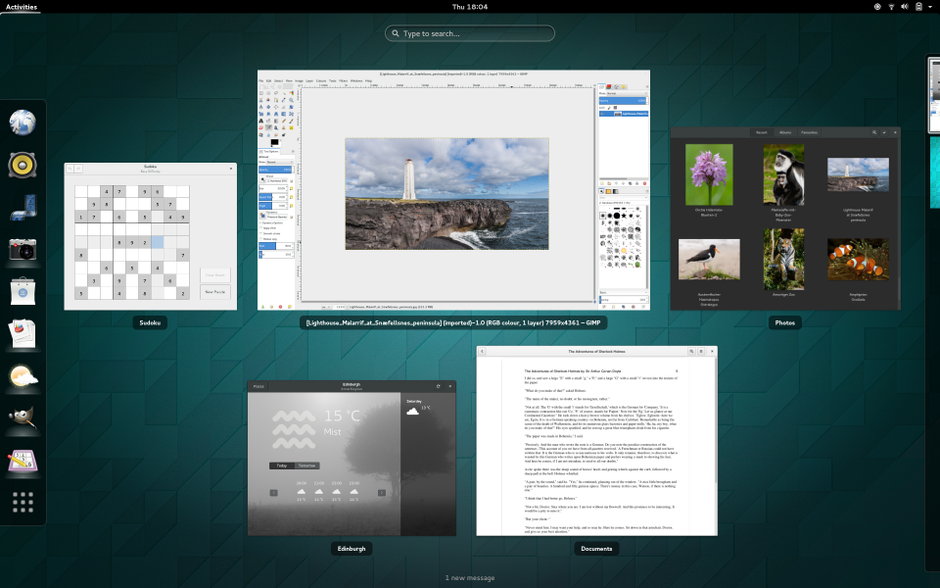
\includegraphics[width=0.65\textwidth]{activities-overview1.png}}
\caption{Gnome application overview \cite{Gnome 3}}
\end{figure}
}

This provides a clean approach, as the user can focus on their application and not on various taskbars and intrusive GUI elements. The aim is simplicity, which is desired for an intuitive touchless navigation experience.	
\item[Architecture]{\hfill \\
The display manager manages access to the desktop and is essentially the login screen, GNOME uses the gnome display manager - GDM. This is launched in the inital script run to define a session, gnome-session. 
This application in turn launches the next and most importnant component, the gnome shell. It provides the base desktop experience, the taskbars, application switcher and launcher as well as coming with gnome applications such as nautilus as it's file manager and a custome settings application for the system called gnome-control-center. It uses a window manager called Mutter, which itself uses a graphical library called Clutter to adjust the layout on screen. There are bindings in all popular languages for comonents across the timeline, with key languages being C++ and javascript. 
}
\item[Customisation]{\hfill \\
Gnome has a prexisting framework for altering it's appearance and behavior. These take the form of small Javascript extensions which have access to both Mutter and Clutter, as well as a way to access the rest of the system. There are bindings to manipulate open windows and make calls to a terminal.
}
\end{description}
\newpage


\subsection{Desktop navigation implementations\label{NavigationExamples}}
There have been a few different implementations of desktop navigation using the Leap, I will examine those availabe open source on Linux and a few paid implementations on windows.
\subsubsectoion{AirInput}
\subsubsection{touchless}
\subsubsection{OSControl applications}
\subsubsection{Pointable}
\subsubsection{Mudra mouse}
\subsubsection{Shortcuts}
\subsubsection{xleapmouse}
\subsubsection{OpenLeap-pyleapmouse}
\subsubsection{leapcursor}
\subsubsection{Leap-Gnome-Controller}
\newpage
\section{Project plan}
My Plan for the project is as follows and I intend to document each step and write the report concurrently as I proceed :

\begin{center}
\begin{tabular}{| p{12cm} |c|}
\hline
Objective & Date due \\
\hline Research architecture and pipeline of the GNOME desktop environment. Decide on which parts of the project are implemented in which languages & $3^{rd}$ April\\
\hline Extend LeapTrainer\cite{LeapTrainer} with SDK v2.x to include more information from the skeletal hand model &$13^{th}$ April \\
\hline Extend LeapTrainer with different gesture recognition algorithms as inspired by examples in the Gesture Recognition Toolkit(GRT) & $20^{th}$ April\\
\hline Perform statistical analysis to find which Gesture recognition algorithm/method is most accurate & $22^{th}$ April \\
\hline
Implement the gesture recognition as a daemon/service and achieve use of it for navigating the desktop in general (Accurate mouse motion, gestures which have some effect on the desktop) & $28^{th}$ April \\
\hline
Implement a method of creating gestures for existing applications- Most likely using configuration files for each application which record sequences of input events to the x server which can be used to send "fake" input events using \texttt{Xlib.ext.xtest} & $8^{th}$ May \\
\hline 
Redefine \texttt{gnome-session} so that the daemon/service starts by default and some basic interactions are loaded by default & $10^{th}$ May \\
\hline
Implement on screen-keyboard with predictive text and Chrome extension to insert LeapCursor\cite{LeapCursor} on every page& $25^{th} May$\\
\hline
Customize look and feel of the \texttt{gnome-shell} so that it's more tailored for the navigation & $4^{th}$ June \\
\hline
Address bugs and redesign interface based on result of user survey & $12^{th}$ June \\
\hline
Address last minute bugs, package up Desktop environment as an installable package(\texttt{.deb}) and finish off report & 16th June \\
\hline
Extension/Fallback : Create custom applications tailored towards the system, file navigator, browser and others. & Unknown \\
\hline
\end{tabular}
\end{center}
 The key objecives are the irst 5 objectives , everything afterwards hinges on completing them. All focus would be on completing them them first and foremost. \\ \\ In particular, the last one "Implement the gesture recognition as a daemon/service and achieve use of it for navigating the desktop in general (Accurate mouse motion, gestures which have some effect on the desktop)" would constitute a partial success in the project, as I would have extended the gesture support for the Leap and would allow other developers to benefit from easier use of the Leap in their applications. If this is completed on time, this would be the halfway point of the project, and the point where the focus of the development would shift to developing the \texttt{GNOME} desktop environment rather than Leap specific work. \\ \\ The next objective would be the next milestone, as it would allow all previous applications to be used intuitively with the Leap. Should this, or the next objective are not met by the $25^{th}$ May, I would shift focus to creating some small applications using the new gesture recognition service, these would either take the form of the applications planned for the completed desktop environment or alternatively as some "Developers tools" or extensions to IDEs. 
 \\ \\ Other extensions could take the shape of abstracting away the Leap specific code to allow it to be used with other tracking devices, altering other desktop environments to be more suited for Leap control.
 \newpage
\section{Evaluation plan}
My first 3 objectives as outlined in section \ref{Objectives} are the most important, and overall (should they be completed on time) constitute  success in the first half of the project. Objectives 4 \& 5 constitute the other half of the project, the side concerned with development of the desktop environment, specifically \texttt{GNOME}. The remaining objectives are extensions in that they are not necessary in order to set the grounds for an intuitive desktop experience using the Leap. 
\subsection{Leap Gesture recognition development and implementation} 
\subsubsection{Objective 1}
I will evaluate my completion of objective one by performing large sets of user tests.Using myself and volunteers , I will record different gestures, of varying complexity, some which will be postures (gestures with no movement). I will evaluate the resultsto see the percentage of the time different gestures are correctly recognized by having the user go through the gestures in a random order. A recognition rate of 80\% or higher would be considered a success as this system would be quite robust. A calibration tool would most likely be created during development, should a user use this, the recognition rate would most likely end up higher anyway.
\subsubsection{Objective 2}
I will assign gestures to various different applications, ranging from web browser, to music software to an email client etc with sequences of actions of varying lengths ranging from one click on a menu button to something with a series of clicks that set print settings and print the page. If it can complete at least 90\% of time (assuming the gesture is recognized(see Objective 1 above)) I will consider this successful and enough to show that any existing application could have gestures assigned to it
\subsubsection{Objective 3}
While integrating the service into the desktop envrionmentwill be easy to evaluate (whether it runs as part of the environment or not) evaluation of the navigation will be composed four parts.
\begin{description}

\item[Mouse accuracy]{\hfill \\
Mouse accuracy will be judged by how intuitive it is to move the mouse and click correctly. If the system is truly intuitive, the user will easily be able to map a point in 3d space, to a point on the monitor. To test this, a test will produce dots at specific locations on screen, the user will be asked to 'click' with the Leap in the location where they think they should to click the dot. Recording the result of where the system actually clicks will give a good measure of the user's accuracy.}
\item[Gestures used to affect navigation]{\hfill \\
This will be judged on a predefined set of gestures which constitute "intuitive" actions in the Desktop Environment. If all actions (for which the gesture has been correctly recognized) are completed correctly this will be considered successful}
\item[2 day user test]{\hfill \\
I will attempt to use the system in place of my every-day computer (this is slightly dependant on objective 5 being completed, however should it not, all keyboard actions will be allowed in the test). If I can use it for 2 days without the need to switch to a mouse, I will deem this test a success. I shall continuously attempt to record my opinions of using the system and any frustrations to properly evaluate this test. }
\item[Survey] {\hfill \\
I will get volunteers to go through versions of the Mouse accuracy and Gestures used to affect navigation set, and ask them to perform some simple everyday tasks. I will get them to fill in a survey based on their experience. Based on their performance in the tests and their opinions of their experience using it, I will be able to assess how well input on the Leap has been implemented } 
\end{description}

\subsection{Development of GnomeLeap}
\subsubsection{Objective 4}
I will judge whether the desktop environment is well tailored towards the Leap based on the user survey from Objective 3 (should it be completed on time). I will ask users their opinions about different menus, how easy the system was to use and whether they had any frustrations. I will keep as many of the questions as quantitative as possible. I will also get the opinion of some lecturers/students from the royal college of arts if possible, as they would have expert input on intuitive design.
\subsubsection{Objective 5}
I will create a typing test, where under a time limit users will type short sentences (short sentences would be the only ones reasonable to use on such a system). Depending on how quickly/accurately users finish each sentence on average will determine how successful the keyboard was. \\
If it is present during the 2 day user test and is used regularly , without switching in a keyboard, will be deemed successful again
\subsection{Extension}
Should I do them, objectives 6 \& 7 will be judged by user survey, asking users opinions on how intuitive the interfaces used are.
\begin{thebibliography} {7}
\bibitem{Leap Site}
Official Leap motion website \texttt{\url{leapmotion.com}}
\bibitem{Leap Overview}
Overview of the Leap system \texttt{\url{https://developer.leapmotion.com/documentation/csharp/devguide/Leap_Overview.html}}
\bibitem{accuracy}
Analysis of the Leap's accuracy
\texttt{Weichert, Frank et al. “Analysis of the Accuracy and Robustness of the Leap Motion Controller.” Sensors (Basel, Switzerland) 13.5 (2013): 6380–6393. PMC. Web. 26 Feb. 2015.}
\bibitem{LeapTrainer}
LeaptTrainer github repository
\texttt{\url{https://github.com/leapmotion/leapjs}}
\bibitem{P}
A gesture recognition algorithm
\texttt{\url{http://faculty.washington.edu/wobbrock/pubs/icmi-12.pdf}}
\bibitem{GRT}
The gesture recognition toolkit
\texttt{\url{http://www.nickgillian.com/software/grt}}
\bibitem{LeapCursor}
LeapCursor github repositor
\texttt{\url{https://github.com/roboleary/LeapCursor.js}}
\bibitem{Leap Teardown}
Video showing what's inside the Leap \texttt{\url{https://www.youtube.com/watch?v=uF0NSUmxFYA}}
\bibitem{Leap Specs}
\texttt{\url{http://en.wikipedia.org/wiki/Leap_Motion\#Technology}}
\bibitem{LeapLab}
Resources for Leap development
\texttt{\url{http://wiki.labomedia.org/index.php/Leap_Motion}}
\bibitem{skeletalGuide}
Developers guide to Leap motion hand model
\texttt{\url{https://developer.leapmotion.com/documentation/csharp/devguide/Intro_Skeleton_API.html}}
\bibitem{devGuide}
Api Overview 
\texttt{\url{https://developer.leapmotion.com/documentation/csharp/devguide/Leap_Overview.html}}
\bibitem{OpenLeapProject}
OpenLeap inititive github
\texttt{\url{https://github.com/openleap}}
\bibitem{OpenLeapDriver}
Github repository for open-source driver attempt for the Leap motion controller
\texttt{\url{https://github.com/openleap/OpenLeap}}
\bibitem{OpenLeapSite}
Openleap  website
\texttt{\url{openleap.org/}}
\bibitem{Gnome}
Gnome project homepage
\texttt{\url{http://www.gnome.org/}}
\bibitem{Gnome 3}
Gnome 3
\texttt{\url{http://www.gnome.org/gnome-3/}}
\end{thebibliography}
\end{document}